\documentclass[12pt,a4paper]{article}
	%[fleqn] %%% --to make all equation left-algned--

% \usepackage[utf8]{inputenc}
% \DeclareUnicodeCharacter{1D12A}{\doublesharp}
% \DeclareUnicodeCharacter{2693}{\anchor}
% \usepackage{dingbat}
% \DeclareRobustCommand\dash\unskip\nobreak\thinspace{\textemdash\allowbreak\thinspace\ignorespaces}
\usepackage[top=2in, bottom=1in, left=1in, right=1in]{geometry}
%\usepackage{fullpage}

\usepackage{fancyhdr}\pagestyle{fancy}\rhead{Stephanie Wang}\lhead{EE236B homework 9}

\usepackage{amsmath,amssymb,amsthm,amsfonts,microtype,stmaryrd}
	%{mathtools,wasysym,yhmath}

\usepackage[usenames,dvipsnames]{xcolor}
\newcommand{\blue}[1]{\textcolor{blue}{#1}}
\newcommand{\red}[1]{\textcolor{red}{#1}}
\newcommand{\gray}[1]{\textcolor{gray}{#1}}
\newcommand{\fgreen}[1]{\textcolor{ForestGreen}{#1}}

\usepackage{mdframed}
	%\newtheorem{mdexample}{Example}
	\definecolor{warmgreen}{rgb}{0.8,0.9,0.85}
	% --Example:
	% \begin{center}
	% \begin{minipage}{0.7\textwidth}
	% \begin{mdframed}[backgroundcolor=warmgreen, 
	% skipabove=4pt,skipbelow=4pt,hidealllines=true, 
	% topline=false,leftline=false,middlelinewidth=10pt, 
	% roundcorner=10pt] 
	%%%% --CONTENTS-- %%%%
	% \end{mdframed}\end{minipage}\end{center}	

\usepackage{graphicx} \graphicspath{{}}
	% --Example:
	% \includegraphics[scale=0.5]{picture name}
%\usepackage{caption} %%% --some awful package to make caption...

\usepackage{hyperref}\hypersetup{linktocpage,colorlinks}\hypersetup{citecolor=black,filecolor=black,linkcolor=black,urlcolor=blue,breaklinks=true}

%%% --Text Fonts
%\usepackage{times} %%% --Times New Roman for LaTeX
%\usepackage{fontspec}\setmainfont{Times New Roman} %%% --Times New Roman; XeLaTeX only

%%% --Math Fonts
\renewcommand{\v}[1]{\ifmmode\mathbf{#1}\fi}
%\renewcommand{\mbf}[1]{\mathbf{#1}} %%% --vector
%\newcommand{\ca}[1]{\mathcal{#1}} %%% --"bigO"
%\newcommand{\bb}[1]{\mathbb{#1}} %%% --"Natural, Real numbers"
%\newcommand{\rom}[1]{\romannumeral{#1}} %%% --Roman numbers

%%% --Quick Arrows
\newcommand{\ra}[1]{\ifnum #1=1\rightarrow\fi\ifnum #1=2\Rightarrow\fi\ifnum #1=3\Rrightarrow\fi\ifnum #1=4\rightrightarrows\fi\ifnum #1=5\rightleftarrows\fi\ifnum #1=6\mapsto\fi\ifnum #1=7\iffalse\fi\fi\ifnum #1=8\twoheadrightarrow\fi\ifnum #1=9\rightharpoonup\fi\ifnum #1=0\rightharpoondown\fi}

%\newcommand{\la}[1]{\ifnum #1=1\leftarrow\fi\ifnum #1=2\Leftarrow\fi\ifnum #1=3\Lleftarrow\fi\ifnum #1=4\leftleftarrows\fi\ifnum #1=5\rightleftarrows\fi\ifnum #1=6\mapsfrom\ifnum #1=7\iffalse\fi\fi\ifnum #1=8\twoheadleftarrow\fi\ifnum #1=9\leftharpoonup\fi\ifnum #1=0\leftharpoondown\fi}

%\newcommand{\ua}[1]{\ifnum #1=1\uparrow\fi\ifnum #1=2\Uparrow\fi}
%\newcommand{\da}[1]{\ifnum #1=1\downarrow\fi\ifnum #1=2\Downarrow\fi}

%%% --Special Editor Config
\renewcommand{\ni}{\noindent}
\newcommand{\onum}[1]{\raisebox{.5pt}{\textcircled{\raisebox{-1pt} {#1}}}}

\newcommand{\claim}[1]{\underline{``{#1}":}}

\renewcommand{\l}{\left}\renewcommand{\r}{\right}

\newcommand{\casebrak}[4]{\left \{ \begin{array}{ll} {#1},&{#2}\\{#3},&{#4} \end{array} \right.}
%\newcommand{\ttm}[4]{\l[\begin{array}{cc}{#1}&{#2}\\{#3}&{#4}\end{array}\r]} %two-by-two-matrix
%\newcommand{\tv}[2]{\l[\begin{array}{c}{#1}\\{#2}\end{array}\r]}

\def\dps{\displaystyle}

\let\italiccorrection=\/
\def\/{\ifmmode\expandafter\frac\else\italiccorrection\fi}


%%% --General Math Symbols
\def\bc{\because}
\def\tf{\therefore}

%%% --Frequently used OPERATORS shorthand
\newcommand{\INT}[2]{\int_{#1}^{#2}}
% \newcommand{\UPINT}{\bar\int}
% \newcommand{\UPINTRd}{\overline{\int_{\bb R ^d}}}
\newcommand{\SUM}[2]{\sum\limits_{#1}^{#2}}
\newcommand{\PROD}[2]{\prod\limits_{#1}^{#2}}
\newcommand{\CUP}[2]{\bigcup\limits_{#1}^{#2}}
\newcommand{\CAP}[2]{\bigcap\limits_{#1}^{#2}}
% \newcommand{\SUP}[1]{\sup\limits_{#1}}
% \newcommand{\INF}[1]{\inf\limits_{#1}}
\DeclareMathOperator*{\argmin}{arg\,min}
\DeclareMathOperator*{\argmax}{arg\,max}
\newcommand{\pd}[2]{\frac{\partial{#1}}{\partial{#2}}}
\def\tr{\text{tr}}

\renewcommand{\o}{\circ}
\newcommand{\x}{\times}
\newcommand{\ox}{\otimes}

\newcommand\ie{{\it i.e. }}
\newcommand\wrt{{w.r.t. }}
\newcommand\dom{\mathbf{dom\:}}

%%% --Frequently used VARIABLES shorthand
\def\R{\ifmmode\mathbb R\fi}
\def\N{\ifmmode\mathbb N\fi}
\renewcommand{\O}{\mathcal{O}}

\newcommand{\dt}{\Delta t}
\def\vA{\mathbf{A}}
\def\vB{\mathbf{B}}\def\cB{\mathcal{B}}
\def\vC{\mathbf{C}}
\def\vD{\mathbf{D}}
\def\vE{\mathbf{E}}
\def\vF{\mathbf{F}}\def\tvF{\tilde{\mathbf{F}}}
\def\vG{\mathbf{G}}
\def\vH{\mathbf{H}}
\def\vI{\mathbf{I}}\def\cI{\mathcal{I}}
\def\vJ{\mathbf{J}}
\def\vK{\mathbf{K}}
\def\vL{\mathbf{L}}\def\cL{\mathcal{L}}
\def\vM{\mathbf{M}}
\def\vN{\mathbf{N}}\def\cN{\mathcal{N}}
\def\vO{\mathbf{O}}
\def\vP{\mathbf{P}}
\def\vQ{\mathbf{Q}}
\def\vR{\mathbf{R}}
\def\vS{\mathbf{S}}
\def\vT{\mathbf{T}}
\def\vU{\mathbf{U}}
\def\vV{\mathbf{V}}
\def\vW{\mathbf{W}}
\def\vX{\mathbf{X}}
\def\vY{\mathbf{Y}}
\def\vZ{\mathbf{Z}}

\def\va{\mathbf{a}}
\def\vb{\mathbf{b}}
\def\vc{\mathbf{c}}
\def\vd{\mathbf{d}}
\def\ve{\mathbf{e}}
\def\vf{\mathbf{f}}
\def\vg{\mathbf{g}}
\def\vh{\mathbf{h}}
\def\vi{\mathbf{i}}
\def\vj{\mathbf{j}}
\def\vk{\mathbf{k}}
\def\vl{\mathbf{l}}
\def\vm{\mathbf{m}}
\def\vn{\mathbf{n}}
\def\vo{\mathbf{o}}
\def\vp{\mathbf{p}}
\def\vq{\mathbf{q}}
\def\vr{\mathbf{r}}
\def\vs{\mathbf{s}}
\def\vt{\mathbf{t}}
\def\vu{\mathbf{u}}
\def\vv{\mathbf{v}}\def\tvv{\tilde{\mathbf{v}}}
\def\vw{\mathbf{w}}
\def\vx{\mathbf{x}}\def\tvx{\tilde{\mathbf{x}}}
\def\vy{\mathbf{y}}
\def\vz{\mathbf{z}}

%%% --Numerical analysis related
%\newcommand{\nxt}{^{n+1}}
%\newcommand{\pvs}{^{n-1}}
%\newcommand{\hfnxt}{^{n+\frac12}}

%%%%%%%%%%%%%%%%%%%%%%%%%%%%%%%%%%%%%%%%%%%%%%%%%%%%%%%%%%%%%%%%%%%%%%%%%%%%%%%%%%%%%%%%%%%%%%%%%%%%%%%%%%%%%%%%%%%%%%%%%%%%%%%%%%%%%%%%%%%%%%%%%%%%%%%%%%%%%%%%%%%%%%%%%%%%%%%%%%%%%%%%%%%%%%%%%%%%%%
\begin{document}
\subsubsection*{Exercise 9.3 [Boyd \& Vandenberghe, 2004]}
{\it Ans:} (a) 
$$p^\ast = \inf_{x_1 >1, x_2 \in \R} x_1^2 + x_2^2 = 1$$
Yet the minimum cannot be attained since we require $x_1 > 1$. \\
\\
(b) Mac built-in Grapher is employed to generate the following graph for the sub-level set $S = \{x \mid f(x) \leq f(x^{(0)})\}$.
\begin{center}
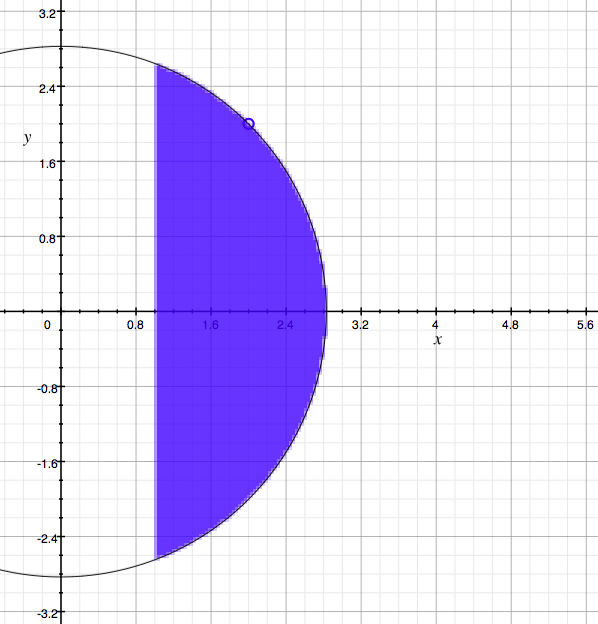
\includegraphics[scale=0.4]{hw9P93.png}
\end{center}
We can see that this is the intersection of the open half-plane $\{x \mid x_1 > 1\}$ with a closed disk $\{x \mid \|x\| \leq \sqrt{8}\}$ which is not closed. On the other hand, $\nabla^2 f = I$ is strongly convex regardless of the domain. \\
\\
(c) We have $\nabla f(x) = 2x$; starting off at $x^{(0)} = (2, 2)$, the gradient will always bring us towards the origin along the line $x_1 = x_2$ since $x^{(k+1)} = x^{(k)} - \alpha_k \nabla f(x^{(k)}) = (1-2\alpha_k) x^{(k)}$. This shows us that the gradient decent method, although implemented with backtracking line search, can only approach a minimum value of $f(1,1) = 2$, which is significantly larger than the actual optimal value $p^\ast = 1$. \qed


\newpage\subsubsection*{Additional Exercise 8.1 [Boyd \& Vandenberghe, 2017]}
{\it Ans:} (a) First from Cauchy's inequality, 
$$x_1y_1 + \sqrt{\gamma}x_2y_2 \leq \sqrt{x_1^2 + \gamma x_2^2}\sqrt{y_1^2+y_2^2} \leq \sqrt{x_1^2 + \gamma x_2^2}$$
This upper bound can be attained when $y_1 = \lambda x_1, y_2 = \lambda \sqrt{\gamma}x_2$. From the constraint $y_1^2 + y_2^2 \leq 1$, we get 
$$\lambda^2(x_1^2+\gamma x_2^2) \leq 1$$
or $\lambda \leq \/1{\sqrt{x_1^2 + \gamma x_2^2}}$. Substituting this result to the constraint $y_1 = \lambda x_1 \geq \/1{\sqrt{1+\gamma}}$, we get 
\begin{align*}
\frac{x_1}{\sqrt{x_1^2 + \gamma x_2^2}} &\geq \/1{\sqrt{1+\gamma}}\\
(1+\gamma)x_1^2 &\geq x_1^2 + \gamma x_2^2 \\
x_1^2 &\geq x_2^2
\end{align*}
Along with the constraint $y_1 \geq \/1{\sqrt{1+\gamma}} > 0$ from which we can induced $x_1 \geq 0$ (o.w. $x_1y_1 \leq 0$ can't make it to the maximum!), we conclude that maximum $\sqrt{x_1^2 + \gamma x_2}$ is attained when 
$$x_1 \geq |x_2|$$
When this constraint is not satisfied, we can see that $\sqrt{\gamma}x_2$ has a larger leverage than $x_1$ in the expression $x_1y_1 + \sqrt{\gamma}x_2y_2$ when we have to balance the weights $y_1, y_2$ due to the constraint $y_1^2 + y_2^2 \leq 1$; therefore to maximize this term, we choose the smallest possible $y_1 = \/1{\sqrt{1+\gamma}}$, then the term is maximized when $y_2 = sgn(x_2)\frac{\sqrt{\gamma}}{\sqrt{1+\gamma}}$ with a value
$$\frac{x_1}{\sqrt{1+\gamma}} + \frac{|x_2|\sqrt{\gamma}}{\sqrt{1+\gamma}}  = \frac{x_1 + |x_2|\sqrt{\gamma}}{\sqrt{1+\gamma}}$$
as desired. Now that $f(x_1, x_2)$ is the supremum of an affine expression over a convex set $D = \{y_1^2 + y_2^2 \leq 1\} \cap \{y_1 \geq 1/\sqrt{1+\gamma}\}$, $f$ itself is a convex function. Note that $f$ is unbounded below since when $x_2 = 0, 0 > x_1 \ra1 -\infty$, 
$$f(x_1, x_2) \leq x_2\sqrt{1+\gamma} \ra1 \infty$$
(b) First we calculate the derivatives of $f$,
$$\pd f{x_1} = \l\{\begin{array}{cc}
\displaystyle\frac{x_1}{\sqrt{x_1^2 + \gamma x_2^2}}, & |x_2|\leq x_1 \\
\displaystyle\frac1{\sqrt{1+\gamma}}, & \mbox{otherwise}
\end{array}\r., 
\pd f{x_2} = \l\{\begin{array}{cc}
\displaystyle\frac{\gamma x_2}{\sqrt{x_1^2 + \gamma x_2^2}}, & |x_2|\leq x_1 \\
\displaystyle\frac{\gamma sgn(x_2)}{\sqrt{1+\gamma}}, & \mbox{otherwise}
\end{array}\r.$$
When we start at $x^{(0)} = (\gamma, 1)$, surely 
$$x_1^{(0)} = \gamma = \gamma\l(\/{\gamma-1}{\gamma+1}\r)^0, x_2^{(0)} = 1 = \l(-\/{\gamma-1}{\gamma+1}\r)^0$$
This forms the base step of the mathematical induction. Now assuming $x_1^{(k)} = \gamma\l(\/{\gamma-1}{\gamma+1}\r)^k, x_2^{(k)} = \l(-\/{\gamma-1}{\gamma+1}\r)^k = \/1\gamma (-1)^k x_1^{(k)}$, then we fall into the case that $|x_2^{(k)}|\leq x_1^{(k)}$ and 
$$\nabla f(x^{(k)}) = \l(\/1{\sqrt{1+\/1\gamma}}, \/{(-1)^k}{\sqrt{1 + \/1\gamma}}\r) = \l(\/{\sqrt{\gamma}}{\sqrt{\gamma+1}}, \/{(-1)^k\sqrt{\gamma}}{\sqrt{\gamma + \gamma}}\r)$$
Here to simply the notation, we denote $L = \/{\gamma-1}{\gamma+1}, H = \sqrt{\/\gamma{\gamma+1}}$, then $x^{(k)} = (\gamma, (-1)^k)L^k , \nabla f(x^{(k)}) = H(1, (-1)^k)$. Now to perform the exact line search, we take the infimum over all possible $t \geq 0$ and complete the square,
\begin{align*}
f(x^{(k)} - t\nabla f(x^{(k)})) &= f(\gamma L^k - tH, (-1)^kL^k - (-1)^ktH)\\
&= \sqrt{(\gamma L^k - tH)^2 + \gamma(L^k - tH)^2} \\
&= \sqrt{\gamma^2 L^{2k} - 2\gamma t L^k H + t^2H^2 + \gamma L^{2k} - 2\gamma tL^kH + \gamma t^2H^2} \\
&= \sqrt{(1+\gamma) H^2 t^2 - 4\gamma t L^k H + (\gamma^2 + \gamma)L^{2k}}\\
&= \sqrt{(1+\gamma) H^2 \l(t-\frac{4\gamma L^k H}{2(1+\gamma) H^2}\r)^2 + (\mbox{some unimportant constant})}
\end{align*}
Hence we get the optimal $t^\ast = \/{2\gamma L^k}{(1+\gamma)H}$ (nonnegative indeed!) and 
\begin{align*}
x^{(k+1)} & = x^{(k)} - \/{2\gamma L^k}{(1+\gamma)H}\nabla f(x^{(k)}) \\
&= \l( \gamma L^k - \/{2\gamma L^k}{1+\gamma}, (-1)^kL^k - (-1)^k \/{2\gamma L^k}{1+\gamma}  \r)\\
&= \l(\gamma L^k \l(1-\/{2}{1+\gamma}\r), (-1)^kL^k\l(1 - \/{2\gamma}{1+\gamma}\r)\r) \\
&= \l(  \gamma L^k \l(\/{\gamma-1}{1+\gamma}\r)  ,  (-1)^k L^k \l(\/{1-\gamma}{1+\gamma}\r) \r) \\
&= (\gamma L^{k+1}, (-1)^{k+1}L^{k+1})
\end{align*}
as desired. Now that $L = \/{\gamma-1}{\gamma+1} < 1$, we know $x^{(k)} = (\gamma, (-1)^k)L^k \ra1 0$ as $k \ra1 \infty$. Certainly gradient decent method with exact line search doesn't give correct optimum for this problem. \qed


\newpage\subsubsection*{Additional Exercise 8.9 [Boyd \& Vandenberghe, 2017]}
{\it Ans:} (a) Define 
$$Q(s) = \/1{\sqrt{2\pi}}\INT{-\infty}{s} e^{-\/{t^2}2}dt$$
In homework 3, {\bf Exercise 3.55 [Boyd \& Vandenberghe]}, we proved this would a log-concave function since $h(t) = \/{t^2}2$ is convex. Now we can write the objective function in terms of $Q$,
$$l(x) = \SUM{b_i - a_i^Tx \leq 0}{} \log(1-Q(b_i - a_i^Tx)) + \SUM{b_i - a_i^Tx > 0}{} \log Q(b_i - a_i^Tx)$$
Another observation is for $1-Q(s) = Q(-s)$ since $e^{-\/{t^2}2}$ is an even function; if we let $\tilde a_i^T = sgn(b_i-a_i^Tx)a_i^T$, $\tilde b_i = sgn(b_i-a_i^Tx)\tilde b_i$, then objective function can be further rewritten
$$l(x) = \SUM{i=1}m \log Q(\tilde b_i - \tilde a_i^Tx)$$
as a sum of concave functions composite affine functions on $x$, which is concave. \\
\\
(b) To apply Newton's method on this problem, we first calculate the gradient and Hessian of the objective function $f(x) = -l(x)$. Denote $z = \tilde b-\tilde Ax$ for simplicity. 
\begin{align*}
\nabla f(x) &= -\SUM{i=1}m \/{Q'(\tilde b_i-\tilde a_i^Tx)}{Q(\tilde b_i-\tilde a_i^Tx)}(-\tilde a_i)\\
&= \SUM{i=1}m \/{e^{-z_i^2/2}}{\INT{-\infty}{z_i} e^{-t^2/2}dt} \tilde a_i\\
&= \SUM{i=1}m \/1{\sqrt{2\pi}\cdot\/12\mathbf{erfcx}(-z_i/\sqrt{2})}\tilde a_i\\
\nabla^2 f(x) &= -\SUM{i=1}m \/{Q''Q - (Q')^2}{Q^2} \tilde a\tilde a^T\\
&= \SUM{i=1}m \/{se^{-\/{s^2}2}\INT{-\infty}s e^{-\/{t^2}2}dt + e^{-s^2}}{\l(\INT{-\infty}s e^{-t^2/2}dt\r)^2}\tilde a_i\tilde a_i^T \\
&= \SUM{i=1}m \l(\/{se^{-s^2/2}}{\INT{-\infty}s e^{-t^2/2}dt} + \l(\/{e^{-s^2/2}}{\INT{-\infty}s e^{-t^2/2}dt}\r)^2 \r)\tilde a_i\tilde a_i^T \\
&= \SUM{i=1}m \l(\/{s}{\sqrt{2\pi}\cdot\/12\mathbf{erfcx}(-s/\sqrt{2})} + \l(\/{1}{\sqrt{2\pi}\cdot\/12\mathbf{erfcx}(-s/\sqrt{2})}\r)^2\r)\tilde a_i\tilde a_i^T
\end{align*}
where $s = \tilde b_i - \tilde a_i^Tx$ in each summand. (Note that from our treatment on coefficients, $\tilde b_i - \tilde a_i^Tx$ is always nonnegative, hence the above Hessian is negative semi-definite, indeed!) The following are two graphs picturing the process of maximizing $l(x)$. Note that I chose the initial guess by random so the graphs look different. I also picked $\alpha = 0.2, \beta = 0.5$. The algorithm usually terminates within about 250 iterations.  \\
Note: I failed many times implementing this algorithm due to the rounding errors introduced by the exponentials. I appreciate how this problem practices me with the MATLAB function \texttt{erfcx}.
\begin{center}
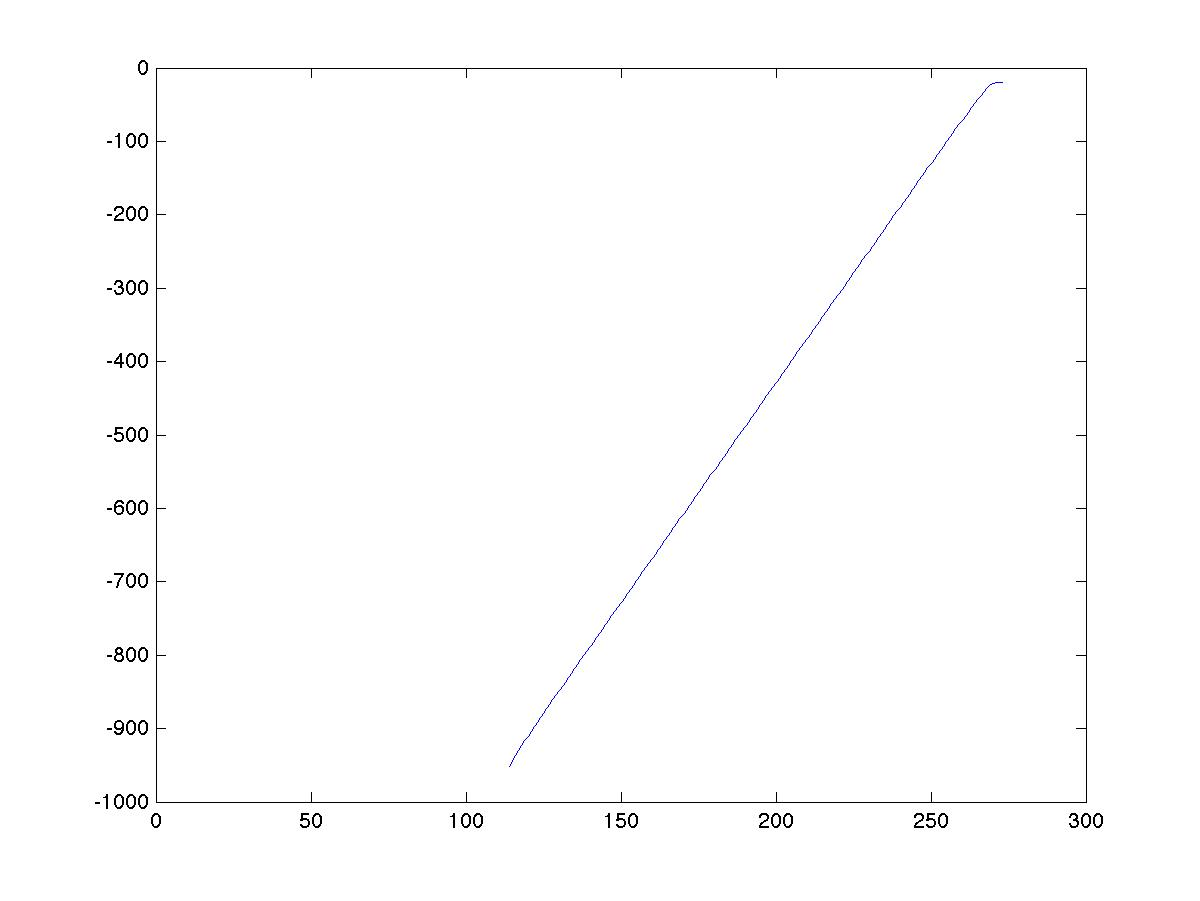
\includegraphics[scale=0.2]{hw9P89.jpg}
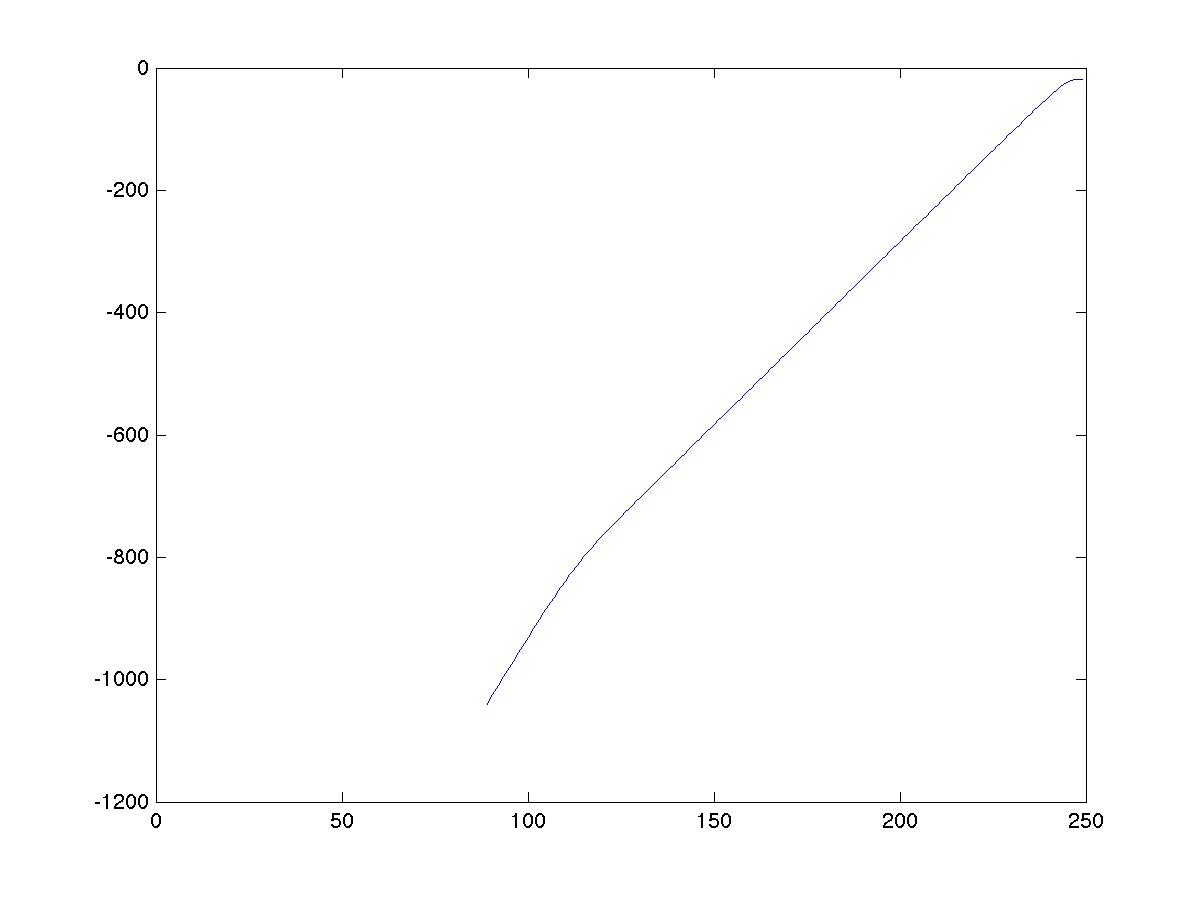
\includegraphics[scale=0.2]{hw9P89-2.jpg}
\end{center}
The optimal solution is around 
\newcommand{\splitatcommas}[1]{%
  \begingroup
  \begingroup\lccode`~=`, \lowercase{\endgroup
    \edef~{\mathchar\the\mathcode`, \penalty0 \noexpand\hspace{0pt plus 1em}}%
  }\mathcode`,="8000 #1%
  \endgroup
}
$x = (\splitatcommas{-0.2708,9.1485,7.9773,6.7027,6.0250,5.0114,4.2996,2.6767,2.0187,0.6842})$. The following is my MATLAB code.
\begin{verbatim}
one_bit_meas_data;
[m,n] = size(A);
for i=1:50
    if y(i) > 0
        A(i,:) = -A(i,:);
        b(i) = -b(i);
        y(i) = -y(i);
    end
end
Q = @(s) 0.5*erfc(-s/sqrt(2));
% dQ = @(s) 1/sqrt(2*pi)*exp(-0.5*s^2);
% ddQ = @(s) -s/sqrt(2*pi)*exp(-0.5*s^2);
l = @(x) sum(log(Q(b-A*x)));
f = @(x) -sum(log(Q(b-A*x)));

max_iter = 1000;
TOL = 1e-3;
alpha = 0.2; %(0.01, 0.3)
beta = 0.5; %(0.1, 0.8)
x = rand(n,1);
for iter = 1:max_iter
    z = b-A*x;
    df = zeros(n,1);
    H = zeros(n);
    for i=1:m
        df = df + sqrt(2/pi)/erfcx(-z(i)/sqrt(2)) * A(i,:)';
        H = H + (z(i)*sqrt(2/pi)/erfcx(-z(i)/sqrt(2)) + (sqrt(2/pi)/erfcx(-z(i)/sqrt(2))^2)) * A(i,:)'*A(i,:);
    end
    dx = - H \ df;
    lsq = df' * (-dx);
    if lsq <= 2*TOL
        break
    end
    t = 1;
    while f(x + t*dx) > f(x) - alpha * t * lsq
        t = beta * t;
    end
    x = x + t * dx;
    x_data(:,iter) = x;
    l_data(iter) = l(x);
end
h1 = plot(1:iter-1,l_data);
saveas(h1,'hw9P89','jpg');
\end{verbatim}






\end{document}



